\documentclass[25pt, blockverticalspace=10mm,  colspace=10mm]{tikzposter}
\tikzposterlatexaffectionproofoff
\geometry{paperwidth=31.1in,paperheight=44in}

\makeatletter
\setlength{\TP@visibletextwidth}{\textwidth-2\TP@innermargin}
\setlength{\TP@visibletextheight}{\textheight-2\TP@innermargin}
\makeatother
% \usepackage{moresize}
\usepackage{graphicx}
% \usepackage[normalem]{ulem}
\usepackage{multirow}
\usepackage{array}
\usepackage{xpatch}
\usepackage[export]{adjustbox}
\usepackage{subfigure}

\usepackage{verbatim}
\usepackage{tikz,times}
\usetikzlibrary{mindmap,backgrounds}
% \pagestyle{empty}

\usepackage{multicol}   
   
\definecolor{darkorange}{rgb}{1.0, 0.35, 0.0}   
\definecolor{darkgreen}{rgb}{0.0, 0.44, 0.0}
\definecolor{columbia}{RGB}{64,104,183}	

\newcommand{\mitem}{{\color{columbia}$\circ$}}
\newcommand{\smitem}{{\color{columbia}--}}

\title{\parbox{\linewidth}{\centering Overview of Commonly-Used Methods to Analyze Exposure to Mixtures \\ in Environmental Epidemiology}} 

\author{Elizabeth A. Gibson$^{{\color{columbia}\dagger}}$, Yanelli Nunez, Marianthi-Anna Kioumourtzoglou}

\institute{
\includegraphics[1.5]{mailman_ehs_4c_horiz.png} \\ \vspace{1ex} {\color{columbia} $^{\dagger}$\url{e.a.gibson@columbia.edu}}}

%\titlegraphic{\includegraphics[scale=.8]{frame.png}}

% \makeatletter
% \renewcommand\TP@maketitle{%
%   \begin{minipage}{0.85\linewidth}
%         \centering
%         \color{titlefgcolor}
%         {\bfseries \huge \sc \@title \par}
%         \vspace*{1em}
%         {\LARGE \@author \par}
%         \vspace*{1em}
%         {\Large \@institute}
%     \end{minipage}%
%     \hfill
%     \begin{minipage}{0.15\linewidth}
%       \centering
%       \@titlegraphic
%     \end{minipage}
% }
% \makeatother

\settitle{ \centering \vbox{
{\bfseries \Huge \@title \par}
\vspace*{1em}
{\huge \@author \par} 
\vspace*{1em} 
{\LARGE \@institute}
}}

\usetheme{Default}
\colorlet{blocktitlebgcolor}{columbia}
\colorlet{framecolor}{columbia}

\begin{document}

\maketitle[width = .95\textwidth]

\block{}{\LARGE

\begin{minipage}[t]{0.47\linewidth}
{\color{white}some random text}
\end{minipage}%
\begin{adjustbox}{valign=t}
\begin{minipage}[l]{0.53\linewidth}
\begin{itemize}
     \item[\mitem] Numerous methods exist for environmental mixtures exposure assessment in health studies 
\begin{itemize}
    \item[\smitem] Developed in other fields or for environmental mixtures 
    \item[\smitem] Choice of method depends on research question(s)
\end{itemize}
    \item[\mitem] We present some {\color{columbia}examples} of commonly-used methods
\begin{itemize}
    \item[\smitem] Grouped by research question
    \end{itemize}
\end{itemize}
\end{minipage}
\end{adjustbox}

\vspace{-10ex}

% \centering
    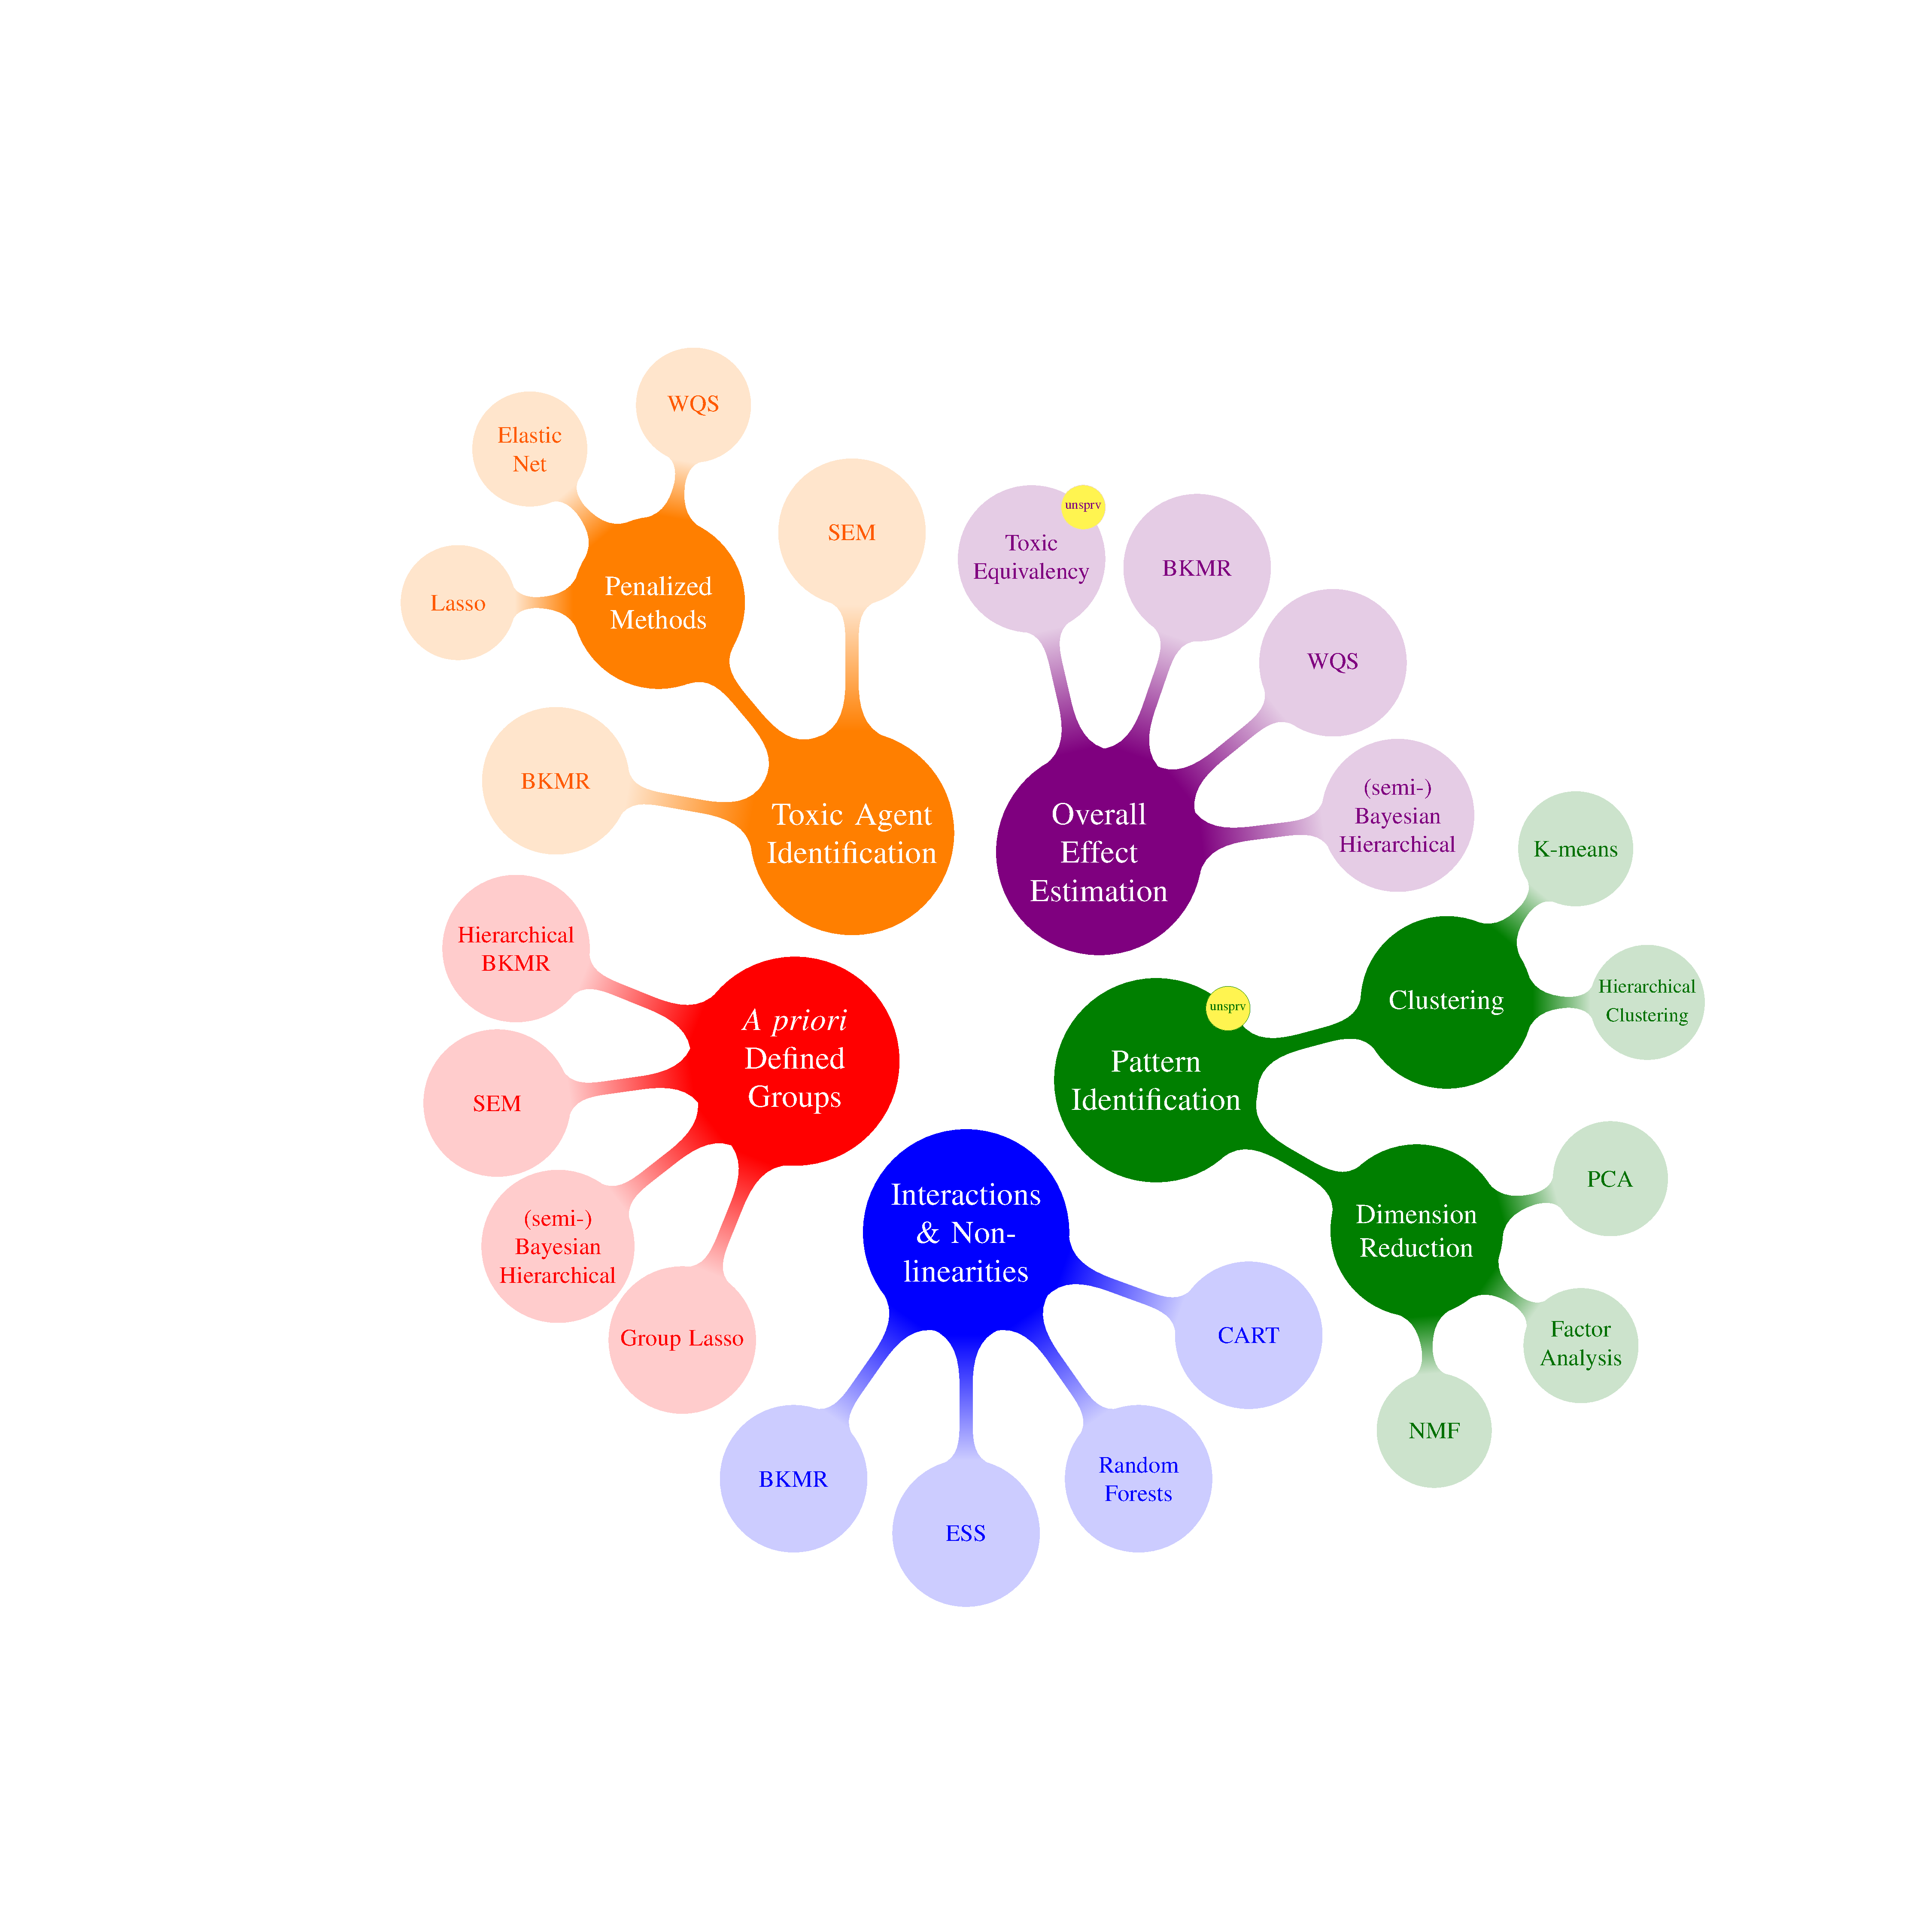
\includegraphics{overview.pdf}

\vspace{-5ex}

{\large
\begin{tabular}{cc}  
  \tikz \node [circle, fill = yellow!80, scale=0.5, ultra thin, draw = black] {unsprv};
  & Unsupervised
  \end{tabular}
}

\vspace{-14ex}

\begin{flushright}
{\Large\color{gray!75}
    \begin{tabular}{ll}
    BKMR    & Bayesian Kernel Machine Regression \\
    CART    & Classification and Regression Trees \\
    ESS     & Exposure Space Smoothing \\
    \multirow{2}{*}{Lasso}   & Least Absolute Shrinkage  \\
            &  and Selection Operator \\
    NFM     & Non-negative Matrix Factorization \\
    PCA     & Principal Component Analysis \\
    SEM     & Structural Equation Modelling \\
    WQS     & Weighted Quantile Sum Regression \\
    \end{tabular}
}    
\end{flushright}

}
\begin{columns}
%\column{0.015}
\column{0.5}


\block{}{\LARGE

\begin{itemize}
\item[\mitem] No single method outperforms all others for {\color{columbia}all} potential questions
\item[\mitem] Other considerations
\begin{enumerate}
\item {\color{columbia} Interpretability}
\item {\color{columbia} Robustness} 
\item Computational scalability 
\begin{itemize}
    \item[\smitem] As dimensionality increases ($N$ or $p$) some methods might start to fail 
\end{itemize}
\item Exploration vs. hypothesis testing
\item Might not be a good idea to ``blindly'' use methods from other fields 
\begin{itemize}
    \item[\smitem] They were developed for different purposes!
    \item[\smitem] May need to adjust them first
\end{itemize}
\end{enumerate}
\end{itemize}


}


\column{0.5}


\block{}{\LARGE
\begin{itemize}
    \item[\mitem] {\color{columbia}To supervise or not to supervise?}
    \begin{enumerate}
        \item Do we want to inform policy?
        \item Or better understand certain biological pathways?
    \end{enumerate}
  \item[\mitem] If (1) {\color{columbia}$\rightarrow$} identify common exposure {\color{columbia} patterns}, independent of outcomes{\color{gray!60}$^{\star}$}, on which we can act 
\begin{itemize}
\item[\smitem] Through regulatory action, interventions etc 
\item[\smitem] E.g. Source apportionment in air pollution
\item[{\color{gray!60}$^{\star}$}] {\normal\color{gray!60} Or rather, to be assessed with many different outcomes}
\end{itemize}
\item[\mitem] If (2) {\color{columbia}$\rightarrow$} of course any method should include the outcome of interest
\end{itemize}


}


\block{}{\centering\Large Support by NIEHS PRIME R01 ES028805, F31 ES030263 \\ and P30 ES009089 \vspace{0.5ex}}


\column{0.015}
\end{columns}
\end{document}

% \block{}{
% \begin{tikzfigure}
% \vspace{-1ex}
% 
\includegraphics[scale = 0.95]{mailman_ehs_4c_horiz.png}
% \vspace{-0.5ex}
% \end{tikzfigure}
% }